%% Part of Stellarium User Guide 0.15+
%% History:
%% 2016-04-17 New chapter.
%% !!!!!!!!!! Please ask GZ before editing this file. !!!!!!!!!!!!!!!


% \chapter{Cultural Astronomy}
% \label{ch:CulturalAstronomy}
% \chapterauthor*{Georg Zotti}
% 
% \noindent \indexterm{Cultural astronomy} describes how astronomy, ritual or
% systematic observation of celestial objects influences the daily life
% of past and present cultures. It encloses astronomical elements of
% calendar making, worship, navigation, celestial mythology, starlore
% and other things not mentioned here.
% 
% Stellarium is a wonderful tool to visualize the sky, celestial
% objects, mythological figures, and the landscape, together describes
% as the \indexterm{skyscape}. The Scenery3D plugin has been described
% in chapter~\ref{ch:Scenery3D}, but apart from this there are more
% extensions which are of interest.
% 
\newpage
\section{ArchaeoLines Plugin}
\label{sec:plugin:ArchaeoLines}
\sectionauthor*{Georg Zotti}
\begin{figure}[ht]
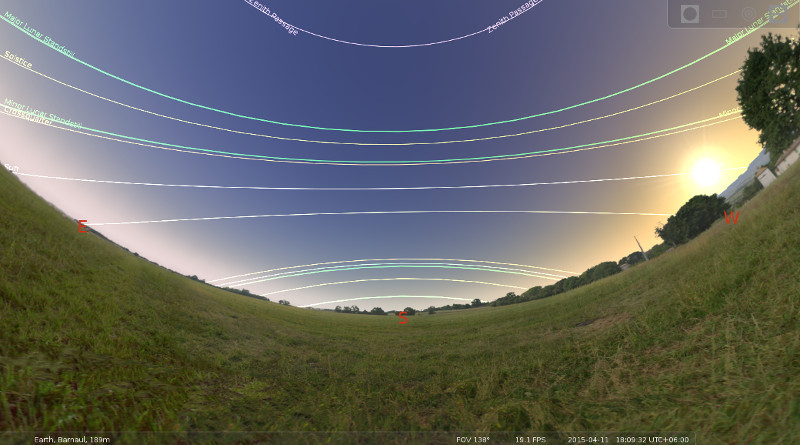
\includegraphics[width=\textwidth,trim=0 50 0 0,clip]{ArchaeoLines.jpg}
\caption{Declination Lines provided by the ArchaeoLines plugin}
\label{fig:plugin:ArchaeoLines}
\end{figure}


\subsection{Introduction}
\label{sec:plugin:ArchaeoLines:Introduction}

In the archaeoastronomical literature, several astronomically derived
orientation schemes are prevalent. Often prehistorical and historical
buildings are described as having been built with a main axis pointing
to a sunrise on summer or winter solstice. There can hardly be a
better tool than Scenery3D (see chapter~\ref{ch:scenery3d}) to
investigate a 3D model of such a building, and this plugin has been
introduced in version 0.13.3 as a further tool in the
archaeoastronomer's toolbox \citep{Zotti:SEAC2015}.

When activated (see section~\ref{sec:Plugins:EnablingPlugins}), you
can find a a tool bar button \guibutton{0.6}{bt_archaeolines.png} (in the
shape of a \emph{trilithon} with the sun shining through it). Press
this, or \key{\ctrl+U}, to display the currently selected set of
characteristical diurnal arcs.

\subsection{Characteristic Declinations}
\label{sec:plugin:ArchaeoLines:Declinations}


The ArchaeoLines plugin displays any combination of declination arcs $\delta$ most
relevant to archaeo- or ethnoastronomical studies. Of course, principles
used in this context are derived from natural observations, and many of
these declinations are still important in everyday astronomy.

\begin{itemize}
\item Declinations of equinoxes (i.e., the equator, $\delta=0$) and the solstices ($\delta=\pm\varepsilon$)
\item Declinations of the crossquarter days (days between solstices and equinoxes, $\delta(\lambda=\pm 45^\circ)$)
\item Declinations of the Major Lunar Standstills ($\delta=\pm(\varepsilon+i)$)
\item Declinations of the Minor Lunar Standstills ($\delta=\pm(\varepsilon-i)$)
\item Declination of the Zenith passage ($\delta=\varphi$)
\item Declination of the Nadir passage ($\delta=-\varphi$)
\item Declination $\delta$ of the currently selected object 
\item Current declination $\delta_{\text{\Sun}}$ of the sun
\item Current declination $\delta_{\text{\Moon}}$ of the moon
\item Current declination $\delta_P$ of a naked-eye planet
\end{itemize}

The principal relation between declinations $\delta$, geographic
latitude $\varphi$, and the rising azimuth $A$ is computed from
\begin{equation}
  \label{eq:RisingAzimuth}
  \cos A=-\frac{\sin\delta}{\cos\varphi}.
\end{equation}

This formula does not take into account local horizon elevation nor
atmospheric refraction nor lunar parallax correction.  The effect
applied to characteristic declinations is shown graphically for the
present time (J2000.0) in
figure~\ref{fig:plugin:ArchaeoLines:MorningLatitudes}. For example, in
a latitude of 30\degree, an object which goes through the zenith rises
at azimuth 55\degree. Lunar major standstill risings occur at azimuths
56.7\degree\ and 123.5\degree, lunar minor standstill risings at
azimuths 69\degree\ and 111\degree. The summer solstice sun rises at
62.6\degree, the winter solstice sun at 117.3\degree. An object which goes
through the nadir rises at 125\degree.  

\begin{figure}[t]
\ifpdf
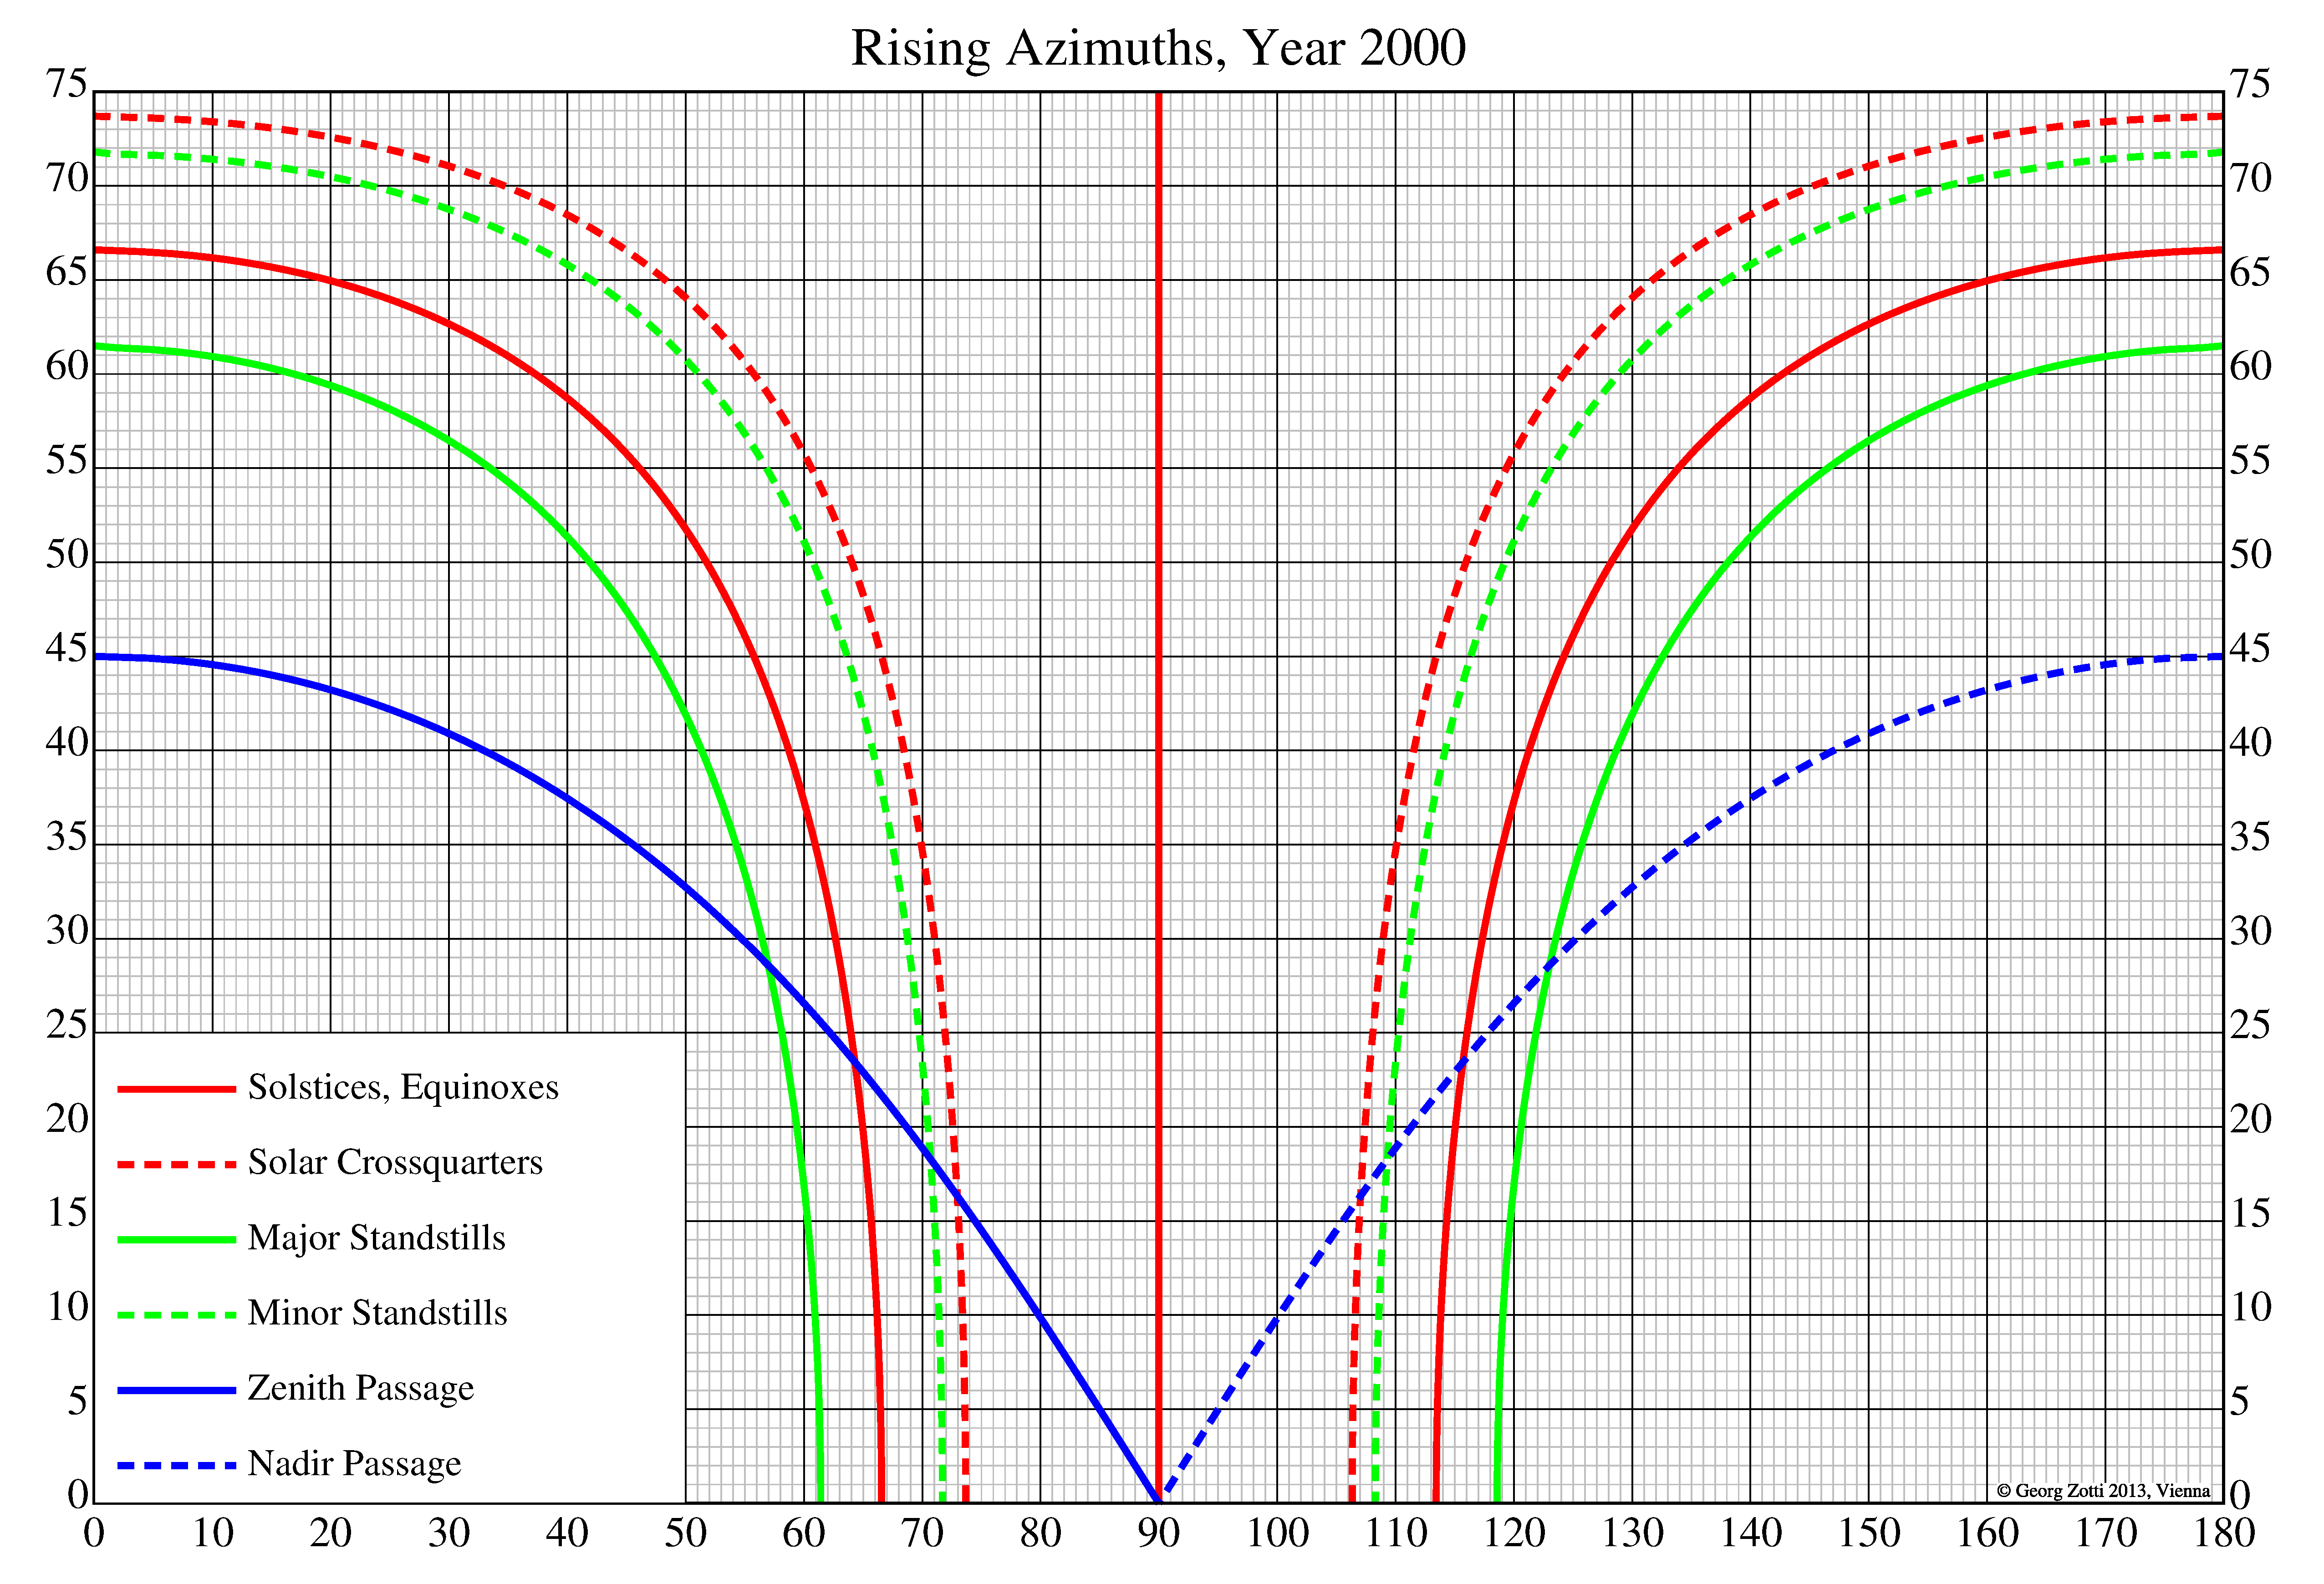
\includegraphics[trim=5 0 5 0,clip,width=\textwidth]{GZ_MorningLatitude}
\else
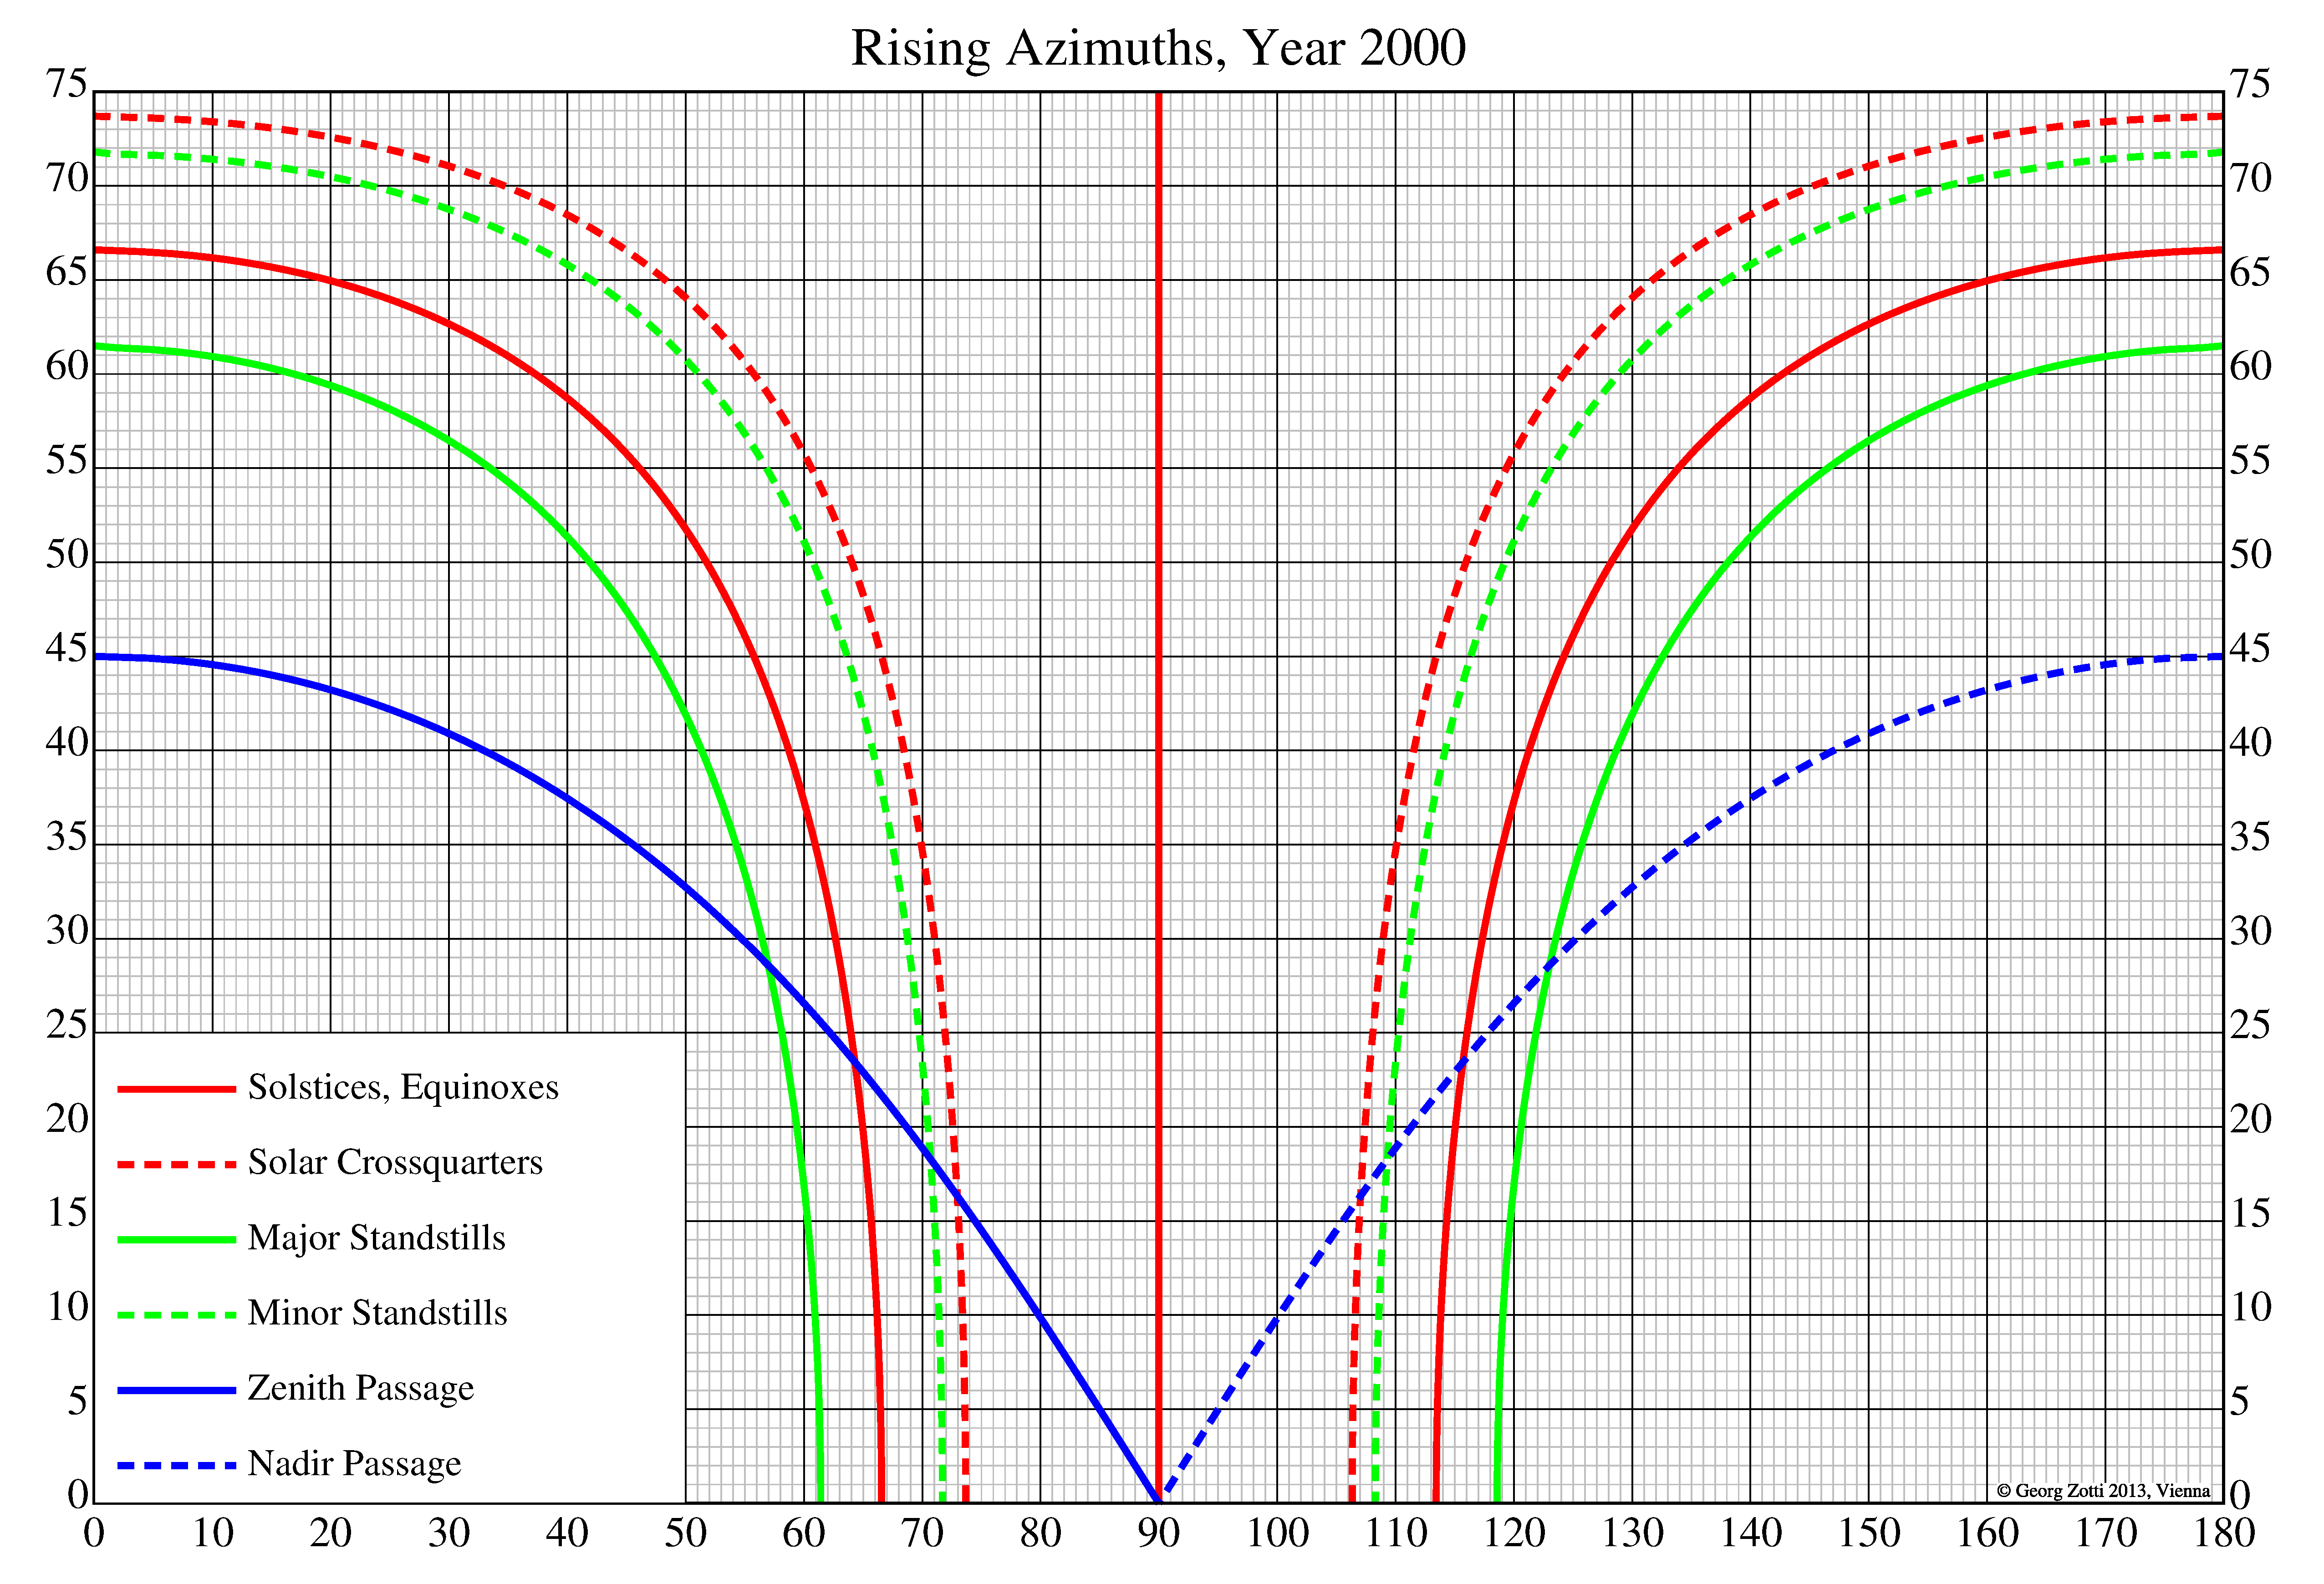
\includegraphics[trim=5 0 5 0,clip,width=\textwidth]{GZ_MorningLatitude.png}
\fi
\caption{Rising azimuths of a few important events for sun and moon,
  and zenith and nadir passages depending on geographic latitudes
  (vertical axis).}
\label{fig:plugin:ArchaeoLines:MorningLatitudes}
\end{figure}

The blue lines seem to vanish at $\varphi=45\degree$: while there are
still objects going through the zenith in higher latitudes, they are
\indexterm{circumpolar} and do not cross the horizon.

For the lunar events, there are two lines each drawn by the plugin,
for maximum and minimum distance of the moon.  The lunar extreme
declinations are computed taking horizon parallax effects into
account. For technical reasons however, the derived declinations are
then used to draw \emph{small circles} of constant declinations on the
sphere, without taking the change of lunar horizontal parallax into
account.  Note that therefore the observed declination of the moon at
the major standstill can exceed the indicated limits if it is high in
the sky. The main purpose of this plugin is however to show an
indication of the intersection of the standstill lines with the
horizon.

It may be very instructive to let the time run quite fast and observe
the declination line of ``current moon'' swinging between its north
and south limits each month.  These limits grow and shrink between the
Major and Minor Standstills in the course of 18.6 years.

The sun likewise swings between the \indexterm[solstice]{solstices}. Over centuries, the
solstice declinations very slightly move as well due to the slightly
changing \indexterm[obliquity, ecliptic]{obliquity of the ecliptic}.

\subsection{Geographical Targets}
\label{sec:plugin:ArchaeoLines:GeographicalTargets}

Some religions, e.g., Islam or Bahai, adhere to a practice of
observing a prayer direction towards a particular location.  Azimuth
lines for two locations can be shown, these lines indicate the great
circle direction towards the locations which can be edited in the
configuration window. Default locations are Mecca (Kaaba) and
Jerusalem.  The azimuth $q$ towards a location $T=(\lambda_T,
\varphi_T)$ can be computed for an observer at $O=(\lambda_O, \varphi_O)$
based on spherical trigonometry on a spherical
Earth~\citep{Abdali:1997} as
\begin{equation}
  \label{eq:qibla}
  q=\arctan \frac{\sin (\lambda_{T} - \lambda_O) } { \cos\varphi_O \tan\varphi_T - \sin\varphi_O \cos(\lambda_{T} - \lambda_O) }
\end{equation}

\noindent You can set \newFeature{0.21.1} geographical coordinates and a name
label directly, or select locations from Stellarium's location list by
pressing the \button{Pick...} button.  You can search for locations in the
list. When you click on a location, its data are taken as target.

\subsection{Custom Lines}
\label{sec:plugin:ArchaeoLines:Custom}

In addition, lines can be shown which indicate arbitrary azimuths (great circles through the zenith),
altitudes, and declinations. \newFeature{0.15.1, 0.21.1}  Note that these azimuths are always counted
from north, regardless of the azimuth setting described in section
\ref{sec:gui:configuration:tools}. These lines can be marked with a custom label.

When some celestial object is selected, you can take over its current
respective data and name by pressing the
\guibutton[0.225]{1.8}{telescope_blk.png} button, however the lines
are \emph{not} linked to the selected objects, and changing angle
values or time will make labels invalid.

\subsection{Configuration Options}
\label{sec:plugin:ArchaeoLines:configuration}

The configuration dialog allows the selection of the lines which are
of interest to you. 
%
%For example, in Mesoamerica the Lunar standstills
%seem not to be relevant, while zenith and nadir passages seem to have
%been important. Also Venus or other planets may appear useful.
%
In addition, you can select the color of the lines by clicking on the
color swatches.
%\footnote{Unfortunately, on some systems with Windows in OpenGL mode, the color dialog hides
%behind the Stellarium window when in fullscreen mode. So, before
%editing line colors, please leave fullscreen mode!}

\subsection*{Section \big[ArchaeoLines\big] in config.ini file}

%Apart from changing settings using the plugin configuration dialog,
%you can also edit the \file{config.ini} file to change
%settings for the ArchaeoLines plugin -- just make it carefully!

\begin{longtable}{l|l|l}\toprule
\emph{ID}                      &\emph{Type} & \emph{Default}  \\\midrule
enable\_at\_startup            &bool        & false           \\
line\_thickness                &int         & 1               \\\midrule
color\_equinox                 &float R,G,B & \ccbox{1.00,1.00,0.50}  \\
color\_solstices               &float R,G,B & \ccbox{1.00,1.00,0.25}  \\
color\_crossquarters           &float R,G,B & \ccbox{1.00,0.75,0.25}  \\
color\_major\_standstill       &float R,G,B & \ccbox{0.25,1.00,0.25}  \\
color\_minor\_standstill       &float R,G,B & \ccbox{0.20,0.75,0.20}  \\
color\_zenith\_passage         &float R,G,B & \ccbox{1.00,0.75,0.75}  \\
color\_nadir\_passage          &float R,G,B & \ccbox{1.00,0.75,0.75}  \\
color\_selected\_object        &float R,G,B & \ccbox{1.00,1.00,1.00}  \\
color\_current\_sun            &float R,G,B & \ccbox{1.00,1.00,0.75}  \\
color\_current\_moon           &float R,G,B & \ccbox{0.50,1.00,0.50}  \\
color\_current\_planet         &float R,G,B & \ccbox{0.25,0.80,1.00}  \\
color\_geographic\_location\_1 &float R,G,B & \ccbox{0.25,1.00,0.25}  \\
color\_geographic\_location\_2 &float R,G,B & \ccbox{0.25,0.25,1.00}  \\
color\_custom\_azimuth\_1      &float R,G,B & \ccbox{0.25,1.00,0.25}  \\
color\_custom\_azimuth\_2      &float R,G,B & \ccbox{0.25,0.50,0.75}  \\
color\_custom\_altitude\_1     &float R,G,B & \ccbox{0.25,1.00,0.25}  \\
color\_custom\_altitude\_2     &float R,G,B & \ccbox{0.25,0.50,0.75}  \\
color\_custom\_declination\_1  &float R,G,B & \ccbox{0.45,1.00,0.15}  \\
color\_custom\_declination\_2  &float R,G,B & \ccbox{0.45,0.50,0.65}  \\\midrule
show\_equinox                  &bool        & true  \\
show\_solstices                &bool        & true  \\
show\_crossquarters            &bool        & true  \\
show\_major\_standstills       &bool        & true  \\
show\_minor\_standstills       &bool        & true  \\
show\_zenith\_passage          &bool        & true  \\
show\_nadir\_passage           &bool        & true  \\
show\_selected\_object         &bool        & true  \\
show\_current\_sun             &bool        & true  \\
show\_current\_moon            &bool        & true  \\
show\_current\_planet          &string      & none  \\\midrule
show\_geographic\_location\_1  &bool        & false         \\
show\_geographic\_location\_2  &bool        & false         \\
geographic\_location\_1\_longitude &double  & 39.826175     \\
geographic\_location\_1\_latitude  &double  & 21.4276       \\
geographic\_location\_1\_label     &string  & Mecca (Qibla) \\
geographic\_location\_2\_longitude &double  & 35.235774     \\
geographic\_location\_2\_latitude  &double  & 31.778087     \\
geographic\_location\_2\_label     &string  & Jerusalem     \\\midrule
show\_custom\_azimuth\_1       &bool        & false    \\
show\_custom\_azimuth\_2       &bool        & false    \\
custom\_azimuth\_1\_angle      &double      & 0.0      \\
custom\_azimuth\_2\_angle      &double      & 0.0      \\
custom\_azimuth\_1\_label      &string      & custAzi1 \\
custom\_azimuth\_2\_label      &string      & custAzi2 \\
show\_custom\_altitude\_1      &bool        & false    \\
show\_custom\_altitude\_2      &bool        & false    \\
custom\_altitude\_1\_angle     &double      & 0.0      \\
custom\_altitude\_2\_angle     &double      & 0.0      \\
custom\_altitude\_1\_label     &string      & custAlt1 \\
custom\_altitude\_2\_label     &string      & custAlt2 \\\midrule
show\_custom\_declination\_1   &bool        & false    \\
show\_custom\_declination\_2   &bool        & false    \\
custom\_declination\_1\_angle  &double      & 0.0      \\
custom\_declination\_1\_label  &string      & custDec1 \\
custom\_declination\_2\_angle  &double      & 0.0      \\
custom\_declination\_2\_label  &string      & custDec2 \\\bottomrule
\end{longtable}

\subsection{Acknowledgements}

If you are using this plugin in scientific publications, please cite \citet{Zotti:SEAC2015}.


%%% Local Variables: 
%%% mode: latex
%%% TeX-master: "guide"
%%% End: 

